\chapter{Classification}

\begin{description}
    \item[(Supervised) classification] \marginnote{Classification} 
        Given a finite set of classes $C$ and a dataset $\matr{X}$ of $N$ individuals, 
        each associated to a class $y(\vec{x}) \in C$,
        we want to learn a model $\mathcal{M}$ able to 
        guess the value of $y(\bar{\vec{x}})$ for unseen individuals.

        Classification can be:
        \begin{descriptionlist}
            \item[Crisp] \marginnote{Crisp classification}
                Each individual has one and only one label.
            \item[Probabilistic] \marginnote{Probabilistic classification}
                Each individual is assigned to a label with a certain probability.
        \end{descriptionlist}

    \item[Classification model] \marginnote{Classification model}
        A classification model (classifier) makes a prediction by taking as input 
        a data element $\vec{x}$ and a decision function $y_\vec{\uptheta}$ parametrized on $\vec{\uptheta}$:
        \[ \mathcal{M}(\vec{x}, \vec{\uptheta}) = y_\vec{\uptheta}(\vec{x}) \]

    \item[Vapnik-Chervonenkis dimension] \marginnote{Vapnik-Chervonenkis dimension}
        A dataset with $N$ elements defines $2^N$ learning problems.
        A model $\mathcal{M}$ has Vapnik-Chervonenkis (VC) dimension $N$ if 
        it is able to solve all the possible learning problems with $N$ elements.

        \begin{example}
            A straight line has VC dimension 3.
        \end{example}

    \item[Data exploration] \marginnote{Data exploration}
        \begin{figure}[ht]
            \begin{subfigure}{.5\textwidth}
                \centering
                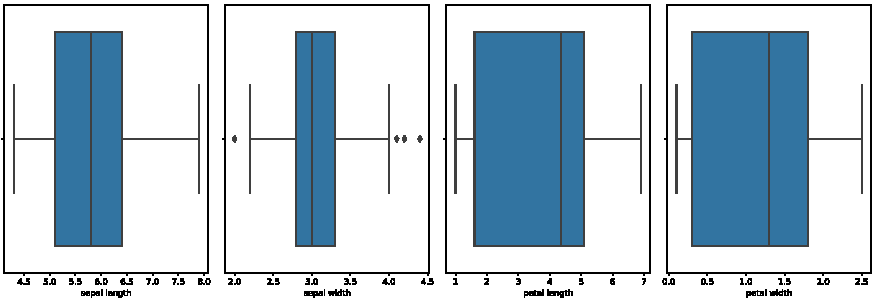
\includegraphics[width=\linewidth]{img/_iris_boxplot_general.pdf}
                \caption{Iris dataset general boxplot}
            \end{subfigure}%
            \begin{subfigure}{.5\textwidth}
                \centering
                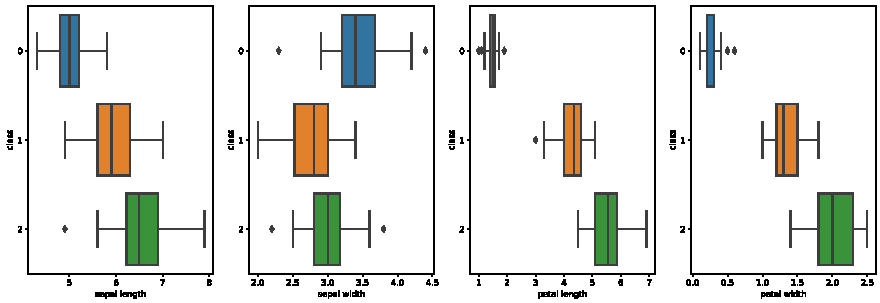
\includegraphics[width=\linewidth]{img/_iris_boxplot_inside.pdf}
                \caption{Iris dataset class boxplot}
            \end{subfigure}
            \begin{subfigure}{.5\textwidth}
                \centering
                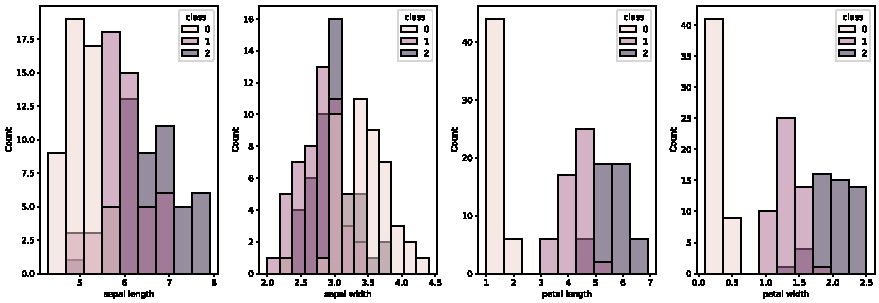
\includegraphics[width=\linewidth]{img/_iris_histogram.pdf}
                \caption{Iris dataset histograms}
            \end{subfigure}%
            \begin{subfigure}{.5\textwidth}
                \centering
                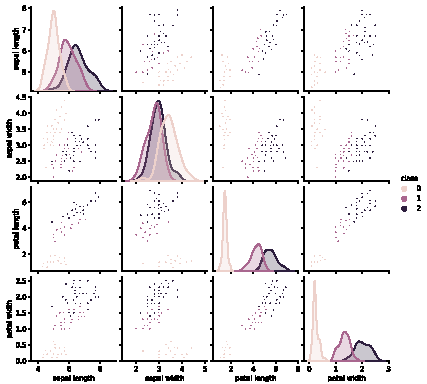
\includegraphics[width=\linewidth]{img/_iris_pairplot.pdf}
                \caption{Iris dataset pairplots}
            \end{subfigure}
        \end{figure}

    \item[Hyperparameters]
        Parameters of the model that have to be manually chosen.
\end{description}


\section{Evaluation}

\begin{description}
    \item[Dataset split]
        A supervised dataset can be randomly split into:
        \begin{descriptionlist}
            \item[Train set] \marginnote{Train set}
                Used to learn the model. Usually the largest split. Can be seen as an upper-bound of the model performance.
            \item[Test set] \marginnote{Test set}
                Used to evaluate the trained model. Can be seen as a lower-bound of the model performance.
            \item[Validation set] \marginnote{Validation set}
                Used to evaluate the model during training and/or for tuning parameters.
        \end{descriptionlist}
        It is assumed that the splits have similar characteristics.

    \item[Overfitting] \marginnote{Overfitting}
        Given a dataset $\matr{X}$, a model $\mathcal{M}$ is overfitting if
        there exists another model $\mathcal{M}'$ such that:
        \[ 
            \begin{split}
                \texttt{error}_\text{train}(\mathcal{M}) &< \texttt{error}_\text{train}(\mathcal{M}') \\
                \texttt{error}_\matr{X}(\mathcal{M}) &> \texttt{error}_\matr{X}(\mathcal{M}') \\
            \end{split}    
        \]

        Possible causes of overfitting are:
        \begin{itemize}
            \item Noisy data.
            \item Lack of representative instances.
        \end{itemize}
\end{description}


\subsection{Test set error}
\textbf{\underline{Disclaimer: I'm very unsure about this part}}\\
The error on the test set can be seen as a lower-bound error of the model.
If the test set error ratio is $x$, we can expect an error of $(x \pm  \text{confidence interval})$.

Predicting the elements of the test set can be seen as a binomial process (i.e. a series of $N$ Bernoulli processes).
We can therefore compute the empirical frequency of success as $f = (\text{correct predictions}/N)$.
We want to estimate the probability of success $p$.

We assume that the deviation between the empirical frequency and the true frequency is due to a 
normal noise around the true probability (i.e. the true probability $p$ is the mean).
Fixed a confidence level $\alpha$ (i.e. the probability of a wrong estimate),
we want that:
\[ \prob{ z_{\frac{\alpha}{2}} \leq \frac{f-p}{\sqrt{\frac{1}{N}p(1-p)}} \leq z_{(1-\frac{\alpha}{2})} } = 1 - \alpha \]
In other words, we want the middle term to have a high probability to 
be between the $\frac{\alpha}{2}$ and $(1-\frac{\alpha}{2})$ quantiles of the gaussian.
\begin{center}
    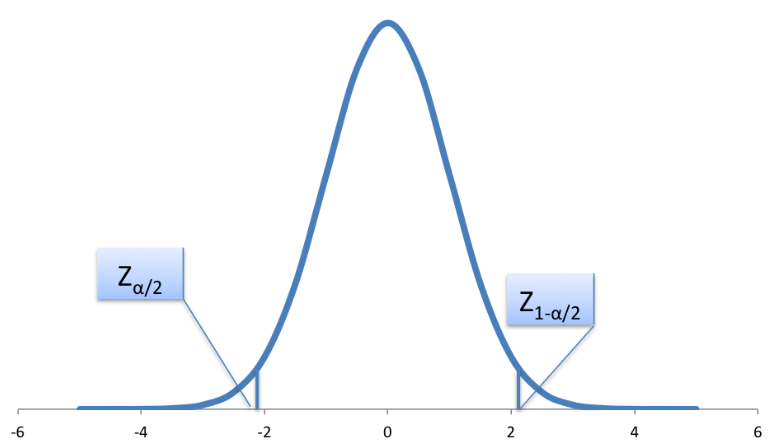
\includegraphics[width=0.35\textwidth]{img/normal_quantile_test_error.png}
\end{center}

We can estimate $p$ using the Wilson score interval\footnote{\url{https://en.wikipedia.org/wiki/Binomial_proportion_confidence_interval}}:
\[ p = \frac{1}{1+\frac{1}{N}z^2} \left( f + \frac{1}{2N}z^2 \pm z\sqrt{\frac{1}{N}f(1-f) + \frac{z^2}{4N^2}} \right) \]
where $z$ depends on the value of $\alpha$.
For a pessimistic estimate, $\pm$ becomes a $+$. Vice versa, for a optimistic estimate, $\pm$ becomes a $-$.

As $N$ is at the denominator, this means that for large values of $N$, the uncertainty becomes smaller.
\begin{center}
    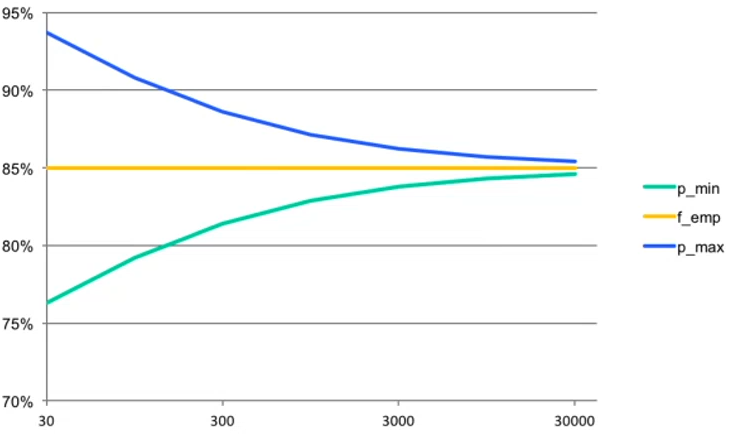
\includegraphics[width=0.45\textwidth]{img/confidence_interval.png}
\end{center}

\subsection{Dataset splits}

\begin{description}
    \item[Holdout] \marginnote{Holdout}
        The dataset is split into train, test and, if needed, validation.

    \item[Cross validation] \marginnote{Cross validation}
        The training data is partitioned into $k$ chunks.
        For $k$ iterations, one of the chunks if used to test and the others to train a new model.
        The overall error is obtained as the average of the errors of the $k$ iterations.

        At the end, the final model is still trained on the entire training data, 
        while cross validation results are used as an evaluation and comparison metric.
        Note that cross validation is done on the training set, so a final test set can still be used to
        evaluate the final model.

        \begin{figure}[h]
            \centering
            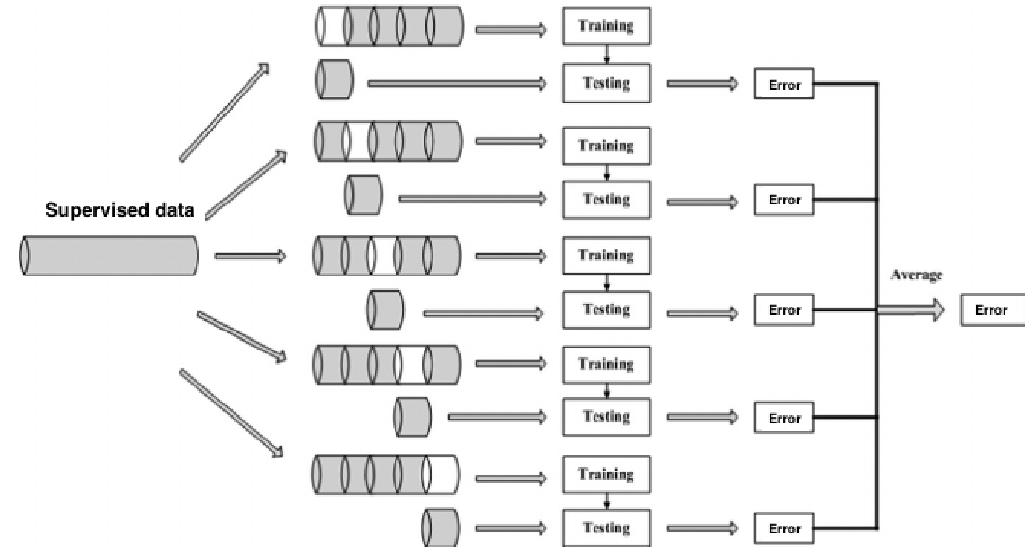
\includegraphics[width=0.6\textwidth]{img/cross_validation.png}
            \caption{Cross validation example}
        \end{figure}

    \item[Leave-one-out] \marginnote{Leave-one-out}
        Extreme case of cross validation with $k=N$, the size of the training set.
        In this case the whole dataset but one element is used for training and the remaining entry for testing.

    \item[Bootstrap] \marginnote{Bootstrap}
        Statistical sampling of the dataset with replacement (i.e. an entry can be selected multiple times).
        The selected entries form the training set while the elements that have never been selected are used for testing.
\end{description}


\subsection{Binary classification performance measures}

In binary classification, the two classes can be distinguished as the positive and negative labels.
The prediction of a classifier can be a:
\begin{center}
    True positive ($TP$) $\cdot$ False positive ($FP$) $\cdot$ True negative ($TN$) $\cdot$ False negative ($FN$)
\end{center}

\begin{center}
    \begin{tabular}{|c|c|c|c|}
        \cline{3-4}
        \multicolumn{2}{c|}{} & \multicolumn{2}{c|}{Predicted} \\
        \cline{3-4}
        \multicolumn{2}{c|}{} & Pos & Neg \\
        \hline
        \multirow{2}{*}{\rotatebox[origin=c]{90}{True}} & Pos & $TP$ & $FN$ \\
        \cline{2-4}
        & Neg & $FP$ & $TN$ \\
        \hline
    \end{tabular}
\end{center}

Given a test set of $N$ element, possible metrics are:
\begin{descriptionlist}
    \item[Accuracy] \marginnote{Accuracy}
        Number of correct predictions.
        \[ \text{accuracy} = \frac{TP + TN}{N} \]

    \item[Error rate] \marginnote{Error rate}
        Number of incorrect predictions.
        \[ \text{error rate} = 1 - \text{accuracy} \]

    \item[Precision] \marginnote{Precision}
        Number of true positives among what the model classified as positive
        (i.e. how many samples the model classified as positive are real positives).
        \[ \text{precision} = \frac{TP}{TP + FP} \]

    \item[Recall/Sensitivity] \marginnote{Recall}
        Number of true positives among the real positives
        (i.e. how many real positive the model predicted).
        \[ \text{recall} = \frac{TP}{TP + FN} \]

    \item[Specificity] \marginnote{Specificity}
        Number of true negatives among the real negatives
        (i.e. recall for negative labels).
        \[ \text{specificity} = \frac{TN}{TN + FP} \]

    \item[F1 score] \marginnote{F1 score}
        Harmonic mean of precision and recall
        (i.e. measure of balance between precision and recall).
        \[ \text{F1} = 2 \frac{\text{precision} \cdot \text{recall}}{\text{precision} + \text{recall}} \]
\end{descriptionlist}


\subsection{Multi-class classification performance measures}

\begin{descriptionlist}
    \item[Confusion matrix] \marginnote{Confusion matrix}
        Matrix to correlate the predictions of $n$ classes:
        \begin{center}
            \begin{tabular}{|c|c|c|c|c|c|}
                \cline{3-6}
                \multicolumn{2}{c|}{} & \multicolumn{4}{c|}{Predicted} \\
                \cline{3-6}
                \multicolumn{2}{c|}{} & a & b & c & Total \\
                \hline
                \multirow{4}{*}{\rotatebox[origin=c]{90}{True}} 
                & a & $TP_a$ & $FP_{a-b}$ & $FP_{a-c}$ & $T_a$ \\
                \cline{2-6}
                & b & $FP_{b-a}$ & $TP_b$ & $FP_{b-c}$ & $T_b$ \\
                \cline{2-6}
                & c & $FP_{c-a}$ & $FP_{c-b}$ & $TP_c$ & $T_c$ \\
                \cline{2-6}
                & Total & $P_a$ & $P_b$ & $P_c$ & $N$ \\
                \hline
            \end{tabular}
        \end{center}
        where:
        \begin{itemize}
            \item $a$, $b$ and $c$ are the classes.
            \item $T_x$ is the true number of labels of class $x$ in the dataset.
            \item $P_x$ is the predicted number of labels of class $x$ in the dataset.
            \item $TP_x$ is the number of times a class $x$ was correctly predicted (true predictions).
            \item $FP_{i-j}$ is the number of times a class $i$ was predicted as $j$ (false predictions).
        \end{itemize}

    \item[Accuracy] \marginnote{Accuracy}
        Accuracy is extended from the binary case as:
        \[ \text{accuracy} = \frac{\sum_i TP_i}{N} \]

    \item[Precision] \marginnote{Precision}
        Precision is defined w.r.t. a single class:
        \[ \text{precision}_i = \frac{TP_i}{P_i} \]

    \item[Recall] \marginnote{Recall}
        Recall is defined w.r.t. a single class:
        \[ \text{recall}_i = \frac{TP_i}{T_i} \]
\end{descriptionlist}

If a single value of precision or recall is needed, the mean can be used by computing
a macro (unweighted) average or a class-weighted average.

\begin{description}
    \item[$\kappa$-statistic] \marginnote{$\kappa$-statistic}
        Evaluates the concordance between two classifiers (in our case, the predictor and the ground truth).
        It is based on two probabilities:
        \begin{descriptionlist}
            \item[Probability of concordance] $\prob{c} = \frac{\sum_{i}^{\texttt{classes}} TP_i}{N}$ 
            \item[Probability of random concordance] $\prob{r} = \frac{\sum_{i}^{\texttt{classes}} T_i P_i}{N^2}$ 
        \end{descriptionlist}

        $\kappa$-statistic is given by:
        \[ \kappa = \frac{\prob{c} - \prob{r}}{1 - \prob{r}} \in [-1, 1] \]
        When $\kappa = 1$, there is perfect agreement ($\sum_{i}^{\texttt{classes}} TP_i = 1$), 
        when $\kappa = -1$, there is total disagreement ($\sum_{i}^{\texttt{classes}} TP_i = 0$) and
        when $\kappa = 0$, there is random agreement.


    \item[Cost sensitive learning] \marginnote{Cost sensitive learning}
        Assign a cost to the errors. This can be done by:
        \begin{itemize}
            \item Altering the proportions of the dataset by duplicating samples to reduce its misclassification.
            \item Weighting the classes (possible in some algorithms).
        \end{itemize}
\end{description}


\subsection{Probabilistic classifier performance measures}

\begin{description}
    \item[Lift chart] \marginnote{Lift chart}
        Used in binary classification.
        Given the resulting probabilities of the positive class of a classifier, 
        sort them in decreasing order and plot a 2d-chart with
        increasing sample size on the x-axis and the number of positive samples on the y-axis.

        Then, plot a straight line to represent a baseline classifier that makes random choices.
        As the probabilities are sorted in decreasing order, it is expected a high concentration of
        positive labels on the right side.
        When the area between the two curves is large and the curve is above the random classifier, 
        the model can be considered a good classifier.

        \begin{figure}[h]
            \centering
            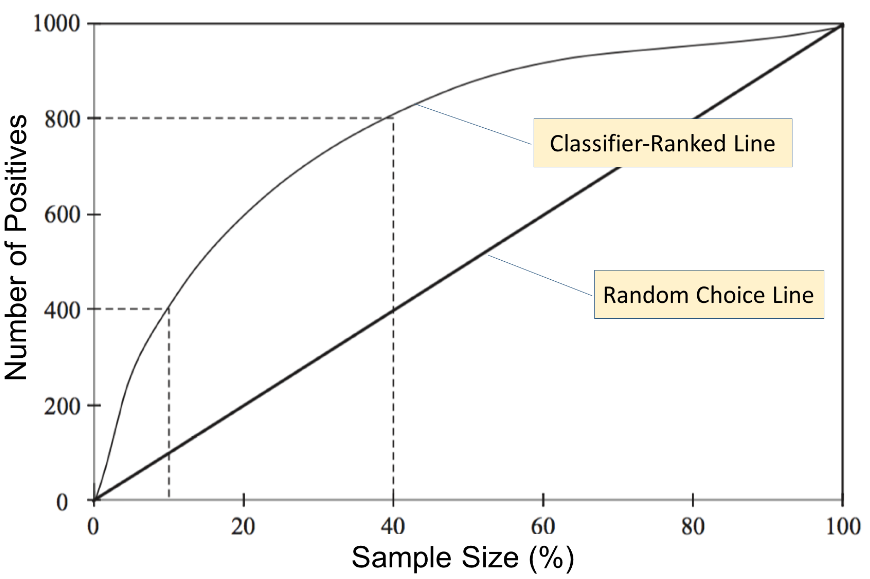
\includegraphics[width=0.5\textwidth]{img/lift_chart.png}
            \caption{Example of lift chart}
        \end{figure}

    \item[ROC curve] \marginnote{ROC curve}
        The ROC curve can be seen as a way to represent multiple confusion matrices of a classifier
        that uses different thresholds.
        The x-axis of a ROC curve represent the false positive rate while the y-axis represent the true positive rate.

        A straight line is used to represent a random classifier.
        A threshold can be considered good if it is high on the y-axis and low on the x-axis.
        
        \begin{figure}[h]
            \centering
            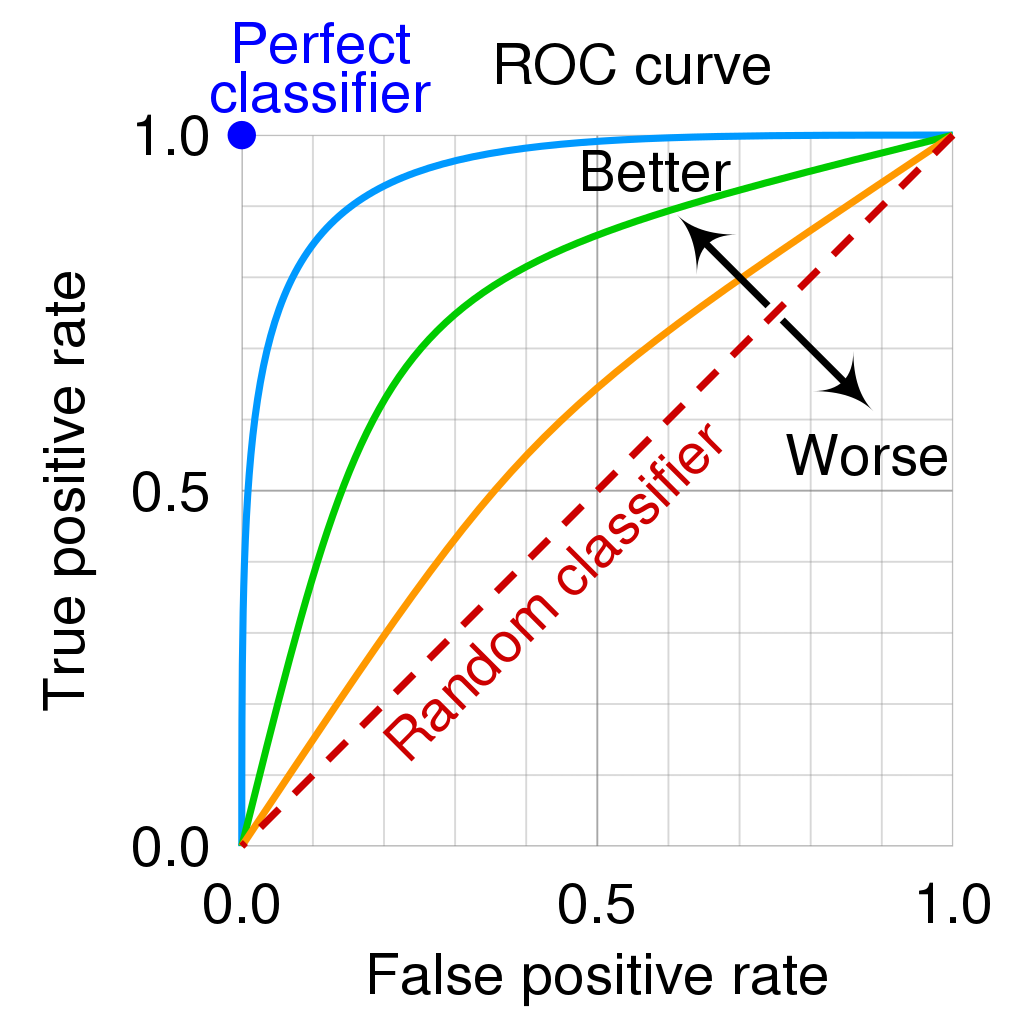
\includegraphics[width=0.35\textwidth]{img/roc_curve.png}
            \caption{Example of ROC curves}
        \end{figure}
\end{description}



\section{Decision trees}

\subsection{Information theory} \label{sec:information_theory}

\begin{description}
    \item[Shannon theorem] \marginnote{Shannon theorem}
        Let $\matr{X} = \{ \vec{v}_1, \dots, \vec{v}_V \}$ be a data source where 
        each of the possible value has probability $p_i = \prob{\vec{v}_i}$.
        The best encoding allows to transmit $\matr{X}$ with 
        an average number of bits given by the \textbf{entropy} of $X$: \marginnote{Entropy}
        \[ H(\matr{X}) = - \sum_j p_j \log_2(p_j) \]
        $H(\matr{X})$ can be seen as a weighted sum of the surprise factor $-\log_2(p_j)$.
        If $p_j \sim 1$, then the surprise of observing $\vec{v}_j$ is low, vice versa,
        if $p_j \sim 0$, the surprise of observing $\vec{v}_j$ is high.
        
        Therefore, when $H(\matr{X})$ is high, $\matr{X}$ is close to an uniform distribution.
        When $H(\matr{X})$ is low, $\matr{X}$ is close to a constant.

        \begin{example}[Binary source] \phantom{}\\
            \begin{minipage}{.50\linewidth}
                The two values of a binary source $\matr{X}$ have respectively probability $p$ and $(1-p)$.
                When $p \sim 0$ or $p \sim 1$, $H(\matr{X}) \sim 0$.\\
                When $p \sim 0.5$, $H(\matr{X}) \sim \log_2(2)=1$
            \end{minipage}
            \begin{minipage}{.45\linewidth}
                \centering
                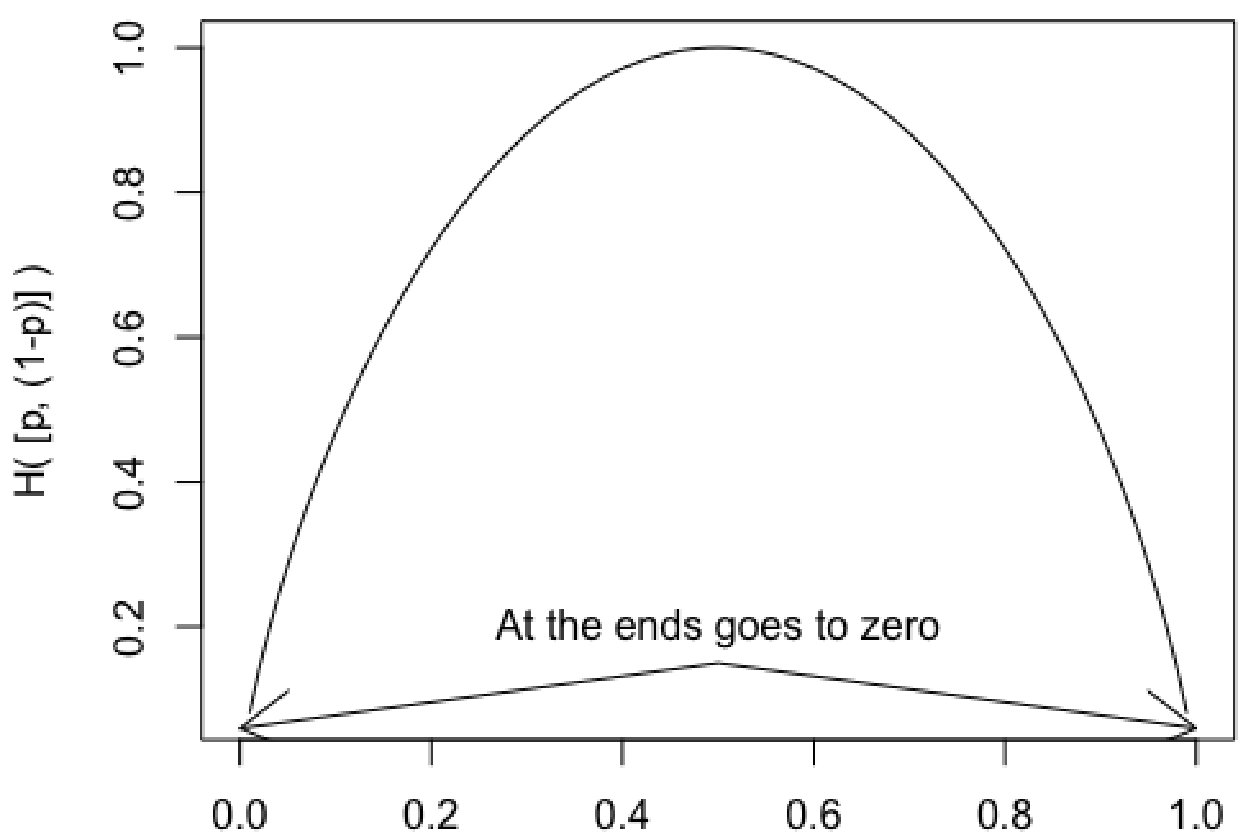
\includegraphics[width=\linewidth]{img/binary_entropy.png}
            \end{minipage}
        \end{example}

    \item[Entropy threshold split] \marginnote{Entropy threshold split}
        Given a dataset $\matr{D}$, 
        a real-valued attribute $d \in \matr{D}$,
        a threshold $t$ in the domain of $d$ and
        the class attribute $c$ of $\matr{D}$.
        The entropy of the class $c$ of the dataset $\matr{D}$ split with threshold $t$ on $d$ is a weighted sum:
        \[ H(c \,\vert\, d \,:\, t) = \prob{d < t}H(c \,\vert\, d < t) + \prob{d \geq t}H(c \,\vert\, d \geq t) \]

    \item[Information gain] \marginnote{Information gain}
        Information gain measures the reduction in entropy after applying a split.
        It is computed as:
        \[ IG(c \,\vert\, d \,:\, t) = H(c) - H(c \,\vert\, d \,:\, t) \]
        When $H(c \,\vert\, d \,:\, t)$ is low, $IG(c \,\vert\, d \,:\, t)$ is high 
        as splitting with threshold $t$ result in purer groups.
        Vice versa, when $H(c \,\vert\, d \,:\, t)$ is high, $IG(c \,\vert\, d \,:\, t)$ is low
        as splitting with threshold $t$ is not very useful.

        The information gain of a class $c$ split on a feature $d$ is given by:
        \[ IG(c \,\vert\, d) = \max_t IG(c \,\vert\, d \,:\, t) \]
\end{description}


\subsection{Tree construction}

\begin{description}
    \item[Decision tree (C4.5)] \marginnote{Decision tree}
        Tree-shaped classifier where leaves are class predictions and 
        inner nodes represent conditions that guide to a leaf.
        This type of classifier is non-linear (i.e. does not represent a linear separation).

        Each node of the tree contains:
        \begin{itemize}
            \item The applied splitting criteria (i.e. feature and threshold). 
                Leaves do not have this value.
            \item The purity (e.g. entropy) of the current split.
            \item Dataset coverage of the current split.
            \item Classes distribution.
        \end{itemize}

        \begin{figure}[h]
            \centering
            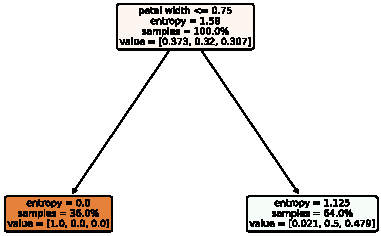
\includegraphics[width=0.5\textwidth]{img/_iris_decision_tree_example.pdf}
            \caption{Example of decision tree}
        \end{figure}

        Note: the weighted sum of the entropies of the children is always smaller than the entropy of the parent.

        Possible stopping conditions are:
        \begin{itemize}
            \item When most of the leaves are pure (i.e. nothing useful to split).
            \item When some leaves are impure but none of the possible splits have positive $IG$.
                Impure leaves are labeled with the majority class.
        \end{itemize}

    \item[Purity] \marginnote{Purity}
        Value to maximize when splitting a node of a decision tree.

        Nodes with uniformly distributed classes have a low purity.
        Nodes with a single class have the highest purity.

        Possible impurity measures are:
        \begin{descriptionlist}
            \item[Entropy/Information gain] See \Cref{sec:information_theory}. 

            \item[Gini index] \marginnote{Gini index}
                Let $\matr{X}$ be a dataset with classes $C$.
                The Gini index measures how often an element of $\matr{X}$ would be misclassified
                if the labels were randomly assigned based on the frequencies of the classes in $\matr{X}$.

                Given a class $i \in C$, $p_i$ is the probability (i.e. frequency) of classifying an element with $i$ and
                $(1 - p_i)$ is the probability of classifying it with a different label.
                The Gini index is given by:
                \[
                    \begin{split}
                        GINI(\matr{X}) = \sum_i^C p_i (1-p_i) &= \sum_i^C p_i - \sum_i^C p_i^2 \\
                            &= 1 - \sum_i^C p_i^2
                    \end{split}  
                \]
                When $\matr{X}$ is uniformly distributed, $GINI(\matr{X}) \sim (1-\frac{1}{\vert C \vert})$.
                When $\matr{X}$ is constant, $GINI(\matr{X}) \sim 0$.

                Given a node $x$ split in $n$ children $x_1, \dots, x_n$,
                the Gini gain of the split is given by:
                \[ GINI_\text{gain} = GINI(x) - \sum_{i=1}^n \frac{\vert x_i \vert}{\vert x \vert} GINI(x_i) \]
 
            \item[Misclassification error] \marginnote{Misclassification error}
                Skipped.
        \end{descriptionlist}

        \begin{figure}[h]
            \centering
            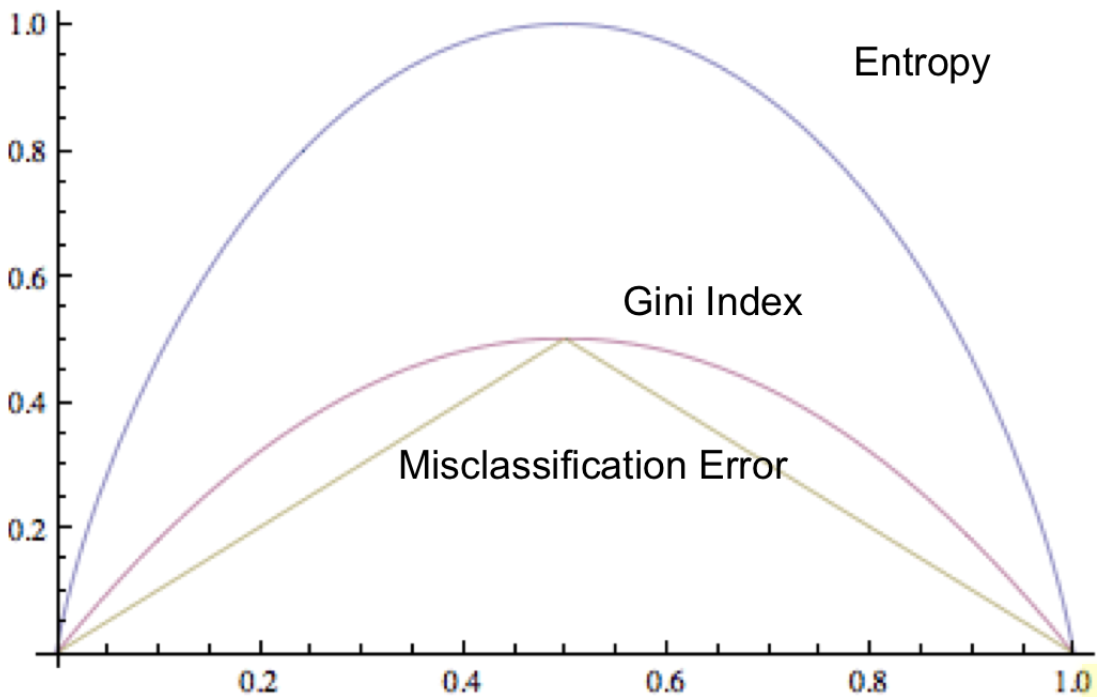
\includegraphics[width=0.35\textwidth]{img/impurity_comparison.png}
            \caption{Comparison of impurity measures}
        \end{figure}

        Compared to Gini index, entropy is more robust to noise.

        Misclassification error has a bias toward the major class.
\end{description}

\begin{algorithm}[H]
\caption{Decision tree construction using information gain as impurity measure}
\begin{lstlisting}
    def buildTree(split):
        node = Node()
        if len(split.classes) == 1: # Pure split
            node.label = split.classes[0]
            node.isLeaf = True
        else:
            ig, attribute, threshold = getMaxInformationGain(split)
            if ig < 0:
                node.label = split.majorityClass()
                node.isLeaf = True
            else:
                node.left = buildTree(split[attribute < threshold])
                node.right = buildTree(split[attribute >= threshold])
        return node
\end{lstlisting}
\end{algorithm}

\begin{description}
    \item[Pruning] \marginnote{Pruning}
        Remove branches to reduce overfitting.
        Different pruning techniques can be employed:
        \begin{descriptionlist}
            \item[Maximum depth] 
                Maximum depth allowed for the tree.

            \item[Minimum samples for split] 
                Minimum number of samples a node is required to have to apply a split.

            \item[Minimum samples for a leaf] 
                Minimum number of samples a node is required to have to become a leaf.

            \item[Minimum impurity decrease] 
                Minimum decrease in impurity for a split to be made.

            \item[Statistical pruning] 
                Prune the children of a node if the weighted sum of the maximum errors of the children is greater than 
                the maximum error of the node if it was a leaf.
        \end{descriptionlist}
\end{description}


\subsection{Complexity}
Given a dataset $\matr{X}$ of $N$ instances and $D$ attributes,
each level of the tree requires to evaluate all the dataset and
each node requires to process all the attributes.
Assuming an average height of $O(\log N)$, 
the overall complexity for induction (parameters search) is $O(DN \log N)$.

Moreover, The other operations of a binary tree have complexity:
\begin{itemize}
    \item Threshold search and binary split: $O(N \log N)$ (scan the dataset for the threshold).
    \item Pruning: $O(N \log N)$ (requires to scan the dataset).
\end{itemize}

For inference, to classify a new instance it is sufficient to traverse the tree from the root to a leaf.
This has complexity $O(h)$, with $h$ the height of the tree.


\subsection{Characteristics}
\begin{itemize}
    \item Decision trees are non-parametric in the sense that they do not require any assumption on the distribution of the data.
    \item Finding the best tree is an NP-complete problem.
    \item Decision trees are robust to noise if appropriate overfitting methods are applied.
    \item Decision trees are robust to redundant attributes (correlated attributes are very unlikely to be chosen for multiple splits).
    \item In practice, the impurity measure has a low impact on the final result, while the pruning strategy is more relevant.
\end{itemize}
